\chapter{Resultados e discussão}
\label{cap:resultados}
% --------------------------------------------------------------------------

A consolidação do arcabouço computacional autônomo culminou na síntese, otimização e qualificação estrutural de uma nova arquitetura de chassi primário para nanossatélites CubeSat 1U em liga aeroespacial AlSi10Mg fabricado por Fusão em Leito de Pó a Laser (L-PBF). Este capítulo apresenta e discute os resultados obtidos nas etapas finais do projeto: (i) a otimização multiobjetivo pelo algoritmo genético NSGA-II acelerado pelo modelo substituto neural \textit{Physics-Guided ResNet}; (ii) a tomada de decisão multicritério pelo método TOPSIS e a caracterização da solução ótima de voo; (iii) a análise de dispersão fonônica por Bloch-Floquet demonstrando a filtragem mecânica por \textit{bandgaps}; (iv) a validação física de alta ordem por simulação em elementos finitos (\textit{FEA Ground Truth}) e convergência de malha; (v) a análise comparativa de desempenho frente ao chassi monolítico convencional; (vi) a qualificação dinâmica ao choque de separação do P-POD e resposta SRS; e (vii) a homologação do espaço de projeto via esteira determinística \textit{open source}.

\section{Otimização multiobjetivo pelo algoritmo NSGA-II e mapeamento da fronteira de Pareto}
\label{sec:nsga}

O problema de otimização de forma e dimensionamento das células metamateriais auxéticas foi formulado com o propósito de mitigar simultaneamente a massa estrutural do chassi e a transmissibilidade dinâmica das acelerações estocásticas transmitidas para a interface da carga útil (\textit{payload}). O problema multiobjetivo restrito é formalizado matematicamente por:
\begin{equation}
  \begin{aligned}
    \min_{\mathbf{x}} \quad & f_1(\mathbf{x}) = m_{\text{total}}(\mathbf{x}) \\
    \min_{\mathbf{x}} \quad & f_2(\mathbf{x}) = T(\mathbf{x}) = \frac{\Grmspay(\mathbf{x})}{\Grmsbase}
  \end{aligned}
  \label{eq:objetivos}
\end{equation}
sujeito ao espaço vetorial de parâmetros geométricos da célula auxética reentrante, $\mathbf{x} = [\theta, t, l, h]^{\top} \in \mathbb{R}^4$:
\begin{equation}
  \begin{aligned}
    \SI{50.0}{\degree} &\le \theta \le \SI{85.0}{\degree} \\
    \SI{0.50}{\milli\metre} &\le t \le \SI{1.80}{\milli\metre} \\
    \SI{6.00}{\milli\metre} &\le l \le \SI{15.00}{\milli\metre} \\
    \SI{8.00}{\milli\metre} &\le h \le \SI{20.00}{\milli\metre}
  \end{aligned}
  \label{eq:limites}
\end{equation}
e às restrições ativas de manufaturabilidade aditiva (DfAM) e integridade espacial (NASA GEVS):
\begin{equation}
  \begin{aligned}
    g_1(\mathbf{x}) &= \theta_{\text{overhang}}(\mathbf{x}) - \SI{35.0}{\degree} \ge 0 \\
    g_2(\mathbf{x}) &= t(\mathbf{x}) - \SI{0.50}{\milli\metre} \ge 0 \\
    g_3(\mathbf{x}) &= d_{\text{drain}}(\mathbf{x}) - \SI{2.00}{\milli\metre} \ge 0 \\
    g_4(\mathbf{x}) &= f_1(\mathbf{x}) - \SI{100.0}{\hertz} \ge 0 \\
    g_5(\mathbf{x}) &= MS_{\text{yield}}(\mathbf{x}) = \left( \frac{\sigma_{\text{adm}}}{\sigma_{3\sigma}(\mathbf{x})} \right) - 1{,}0 \ge 0 \\
    g_6(\mathbf{x}) &= \num{0.25} - D_{\text{Steinberg}}(\mathbf{x}) \ge 0
  \end{aligned}
  \label{eq:restricoes}
\end{equation}
em que $\sigma_{\text{adm}} = \sigma_{\text{yield}} / FS_{\text{yield}} = \SI{230.0}{\mega\pascal} / \num{1.25} = \SI{184.0}{\mega\pascal}$ e o dano cumulativo de fadiga é delimitado pelo critério da NASA-HDBK-7005 (NASA, 2001), $D \le \num{0.25}$.

O conjunto de restrições foi estruturado em dois pilares complementares de engenharia:
\begin{alineas}
  \item \textbf{manufaturabilidade aditiva (DfAM, $g_1$ a $g_3$):} a restrição $g_1$ assegura ângulo de balanço (\textit{overhang}) $\theta_{\text{overhang}} \ge \SI{35.0}{\degree}$, garantindo que todas as costelas oblíquas sejam auto-sustentadas durante o escaneamento a laser sem demandar suportes internos sacrificiais; a restrição $g_2$ impõe espessura mínima de parede $t \ge \SI{0.50}{\milli\metre}$, respeitando a resolução térmica do \textit{spot} do feixe de laser ($\approx \SI{100}{\micro\metre}$) e a granulometria do pó; e a restrição $g_3$ estabelece orifícios de drenagem $d_{\text{drain}} \ge \SI{2.00}{\milli\metre}$ e vão livre intercelular superior a \SI{1.50}{\milli\metre}, assegurando a total evacuação e despoeiramento do pó metálico residual pós-processamento;
  \item \textbf{integridade estrutural e qualificação aeroespacial (NASA GEVS, $g_4$ a $g_6$):} a restrição $g_4$ blinda o satélite contra ressonância dinâmica primária ao impor $f_1 \ge \SI{100.0}{\hertz}$; a restrição $g_5$ impõe margem de segurança estritamente não-negativa ($MS_{\text{yield}} \ge 0$) sob solicitação estocástica a $3\sigma$, com fator de segurança estrutural de qualificação $FS_{\text{yield}} = \num{1.25}$; e a restrição $g_6$ limita o dano de fadiga aleatória acumulada pelo método das três bandas de Steinberg a $D \le \num{0.25}$, provendo margem de vida em fadiga de quatro vezes frente à qualificação de voo.
\end{alineas}

A busca evolutiva operou com uma população de $N_{\text{pop}} = 100$ indivíduos ao longo de $N_{\text{gen}} = 100$ gerações, totalizando \num{10000} avaliações completas de candidatos. O algoritmo utilizou operadores de cruzamento binário simulado (SBX, com índice de distribuição $\eta_c = 15$ e probabilidade de recombinação $p_c = \num{0.90}$), mutação polinomial ($\eta_m = 20$ e $p_m = \num{0.25}$) e o mecanismo de ordenação por dominância restrita de Deb (\textit{Deb's Constrained Domination}) (DEB \textit{et al.}, 2002), o qual confere prioridade absoluta aos indivíduos factíveis e penaliza soluções inviáveis proporcionalmente à sua violação agregada de restrições.

Graças à substituição do solver numérico pela inferência ultrarrápida da rede neural residual guiada por física (\textit{Physics-Guided ResNet}), que registrou latência média de apenas \SI{0.405}{\milli\second} por indivíduo, a campanha evolutiva completa de \num{10000} avaliações foi executada em apenas \textbf{\SI{4.82}{\second}}. Em contrapartida, a mesma varredura executada diretamente no solver Ansys MAPDL (a um custo médio de \SI{100.0}{\second} por análise tridimensional com elementos SOLID187) demandaria cerca de \textbf{\SI{277.8}{\hour} de processamento contínuo} (mais de 11 dias ininterruptos). Esse contraste atesta a aceleração de mais de \num{200000} vezes ($\approx \num{247000}\times$) viabilizada pelo metamodelo neural.

Ao final das 100 gerações, mapeou-se um conjunto de 100 soluções Pareto-ótimas estritamente factíveis, cuja distribuição e correlações estruturais estão ilustradas na Figura~\ref{fig:pareto}.

\begin{figure}[htb]
  \caption{Fronteira de Pareto multiobjetivo (massa estrutural $\times$ transmissibilidade dinâmica) e correlações paramétricas obtidas pelo algoritmo NSGA-II}
  \label{fig:pareto}
  \begin{center}
    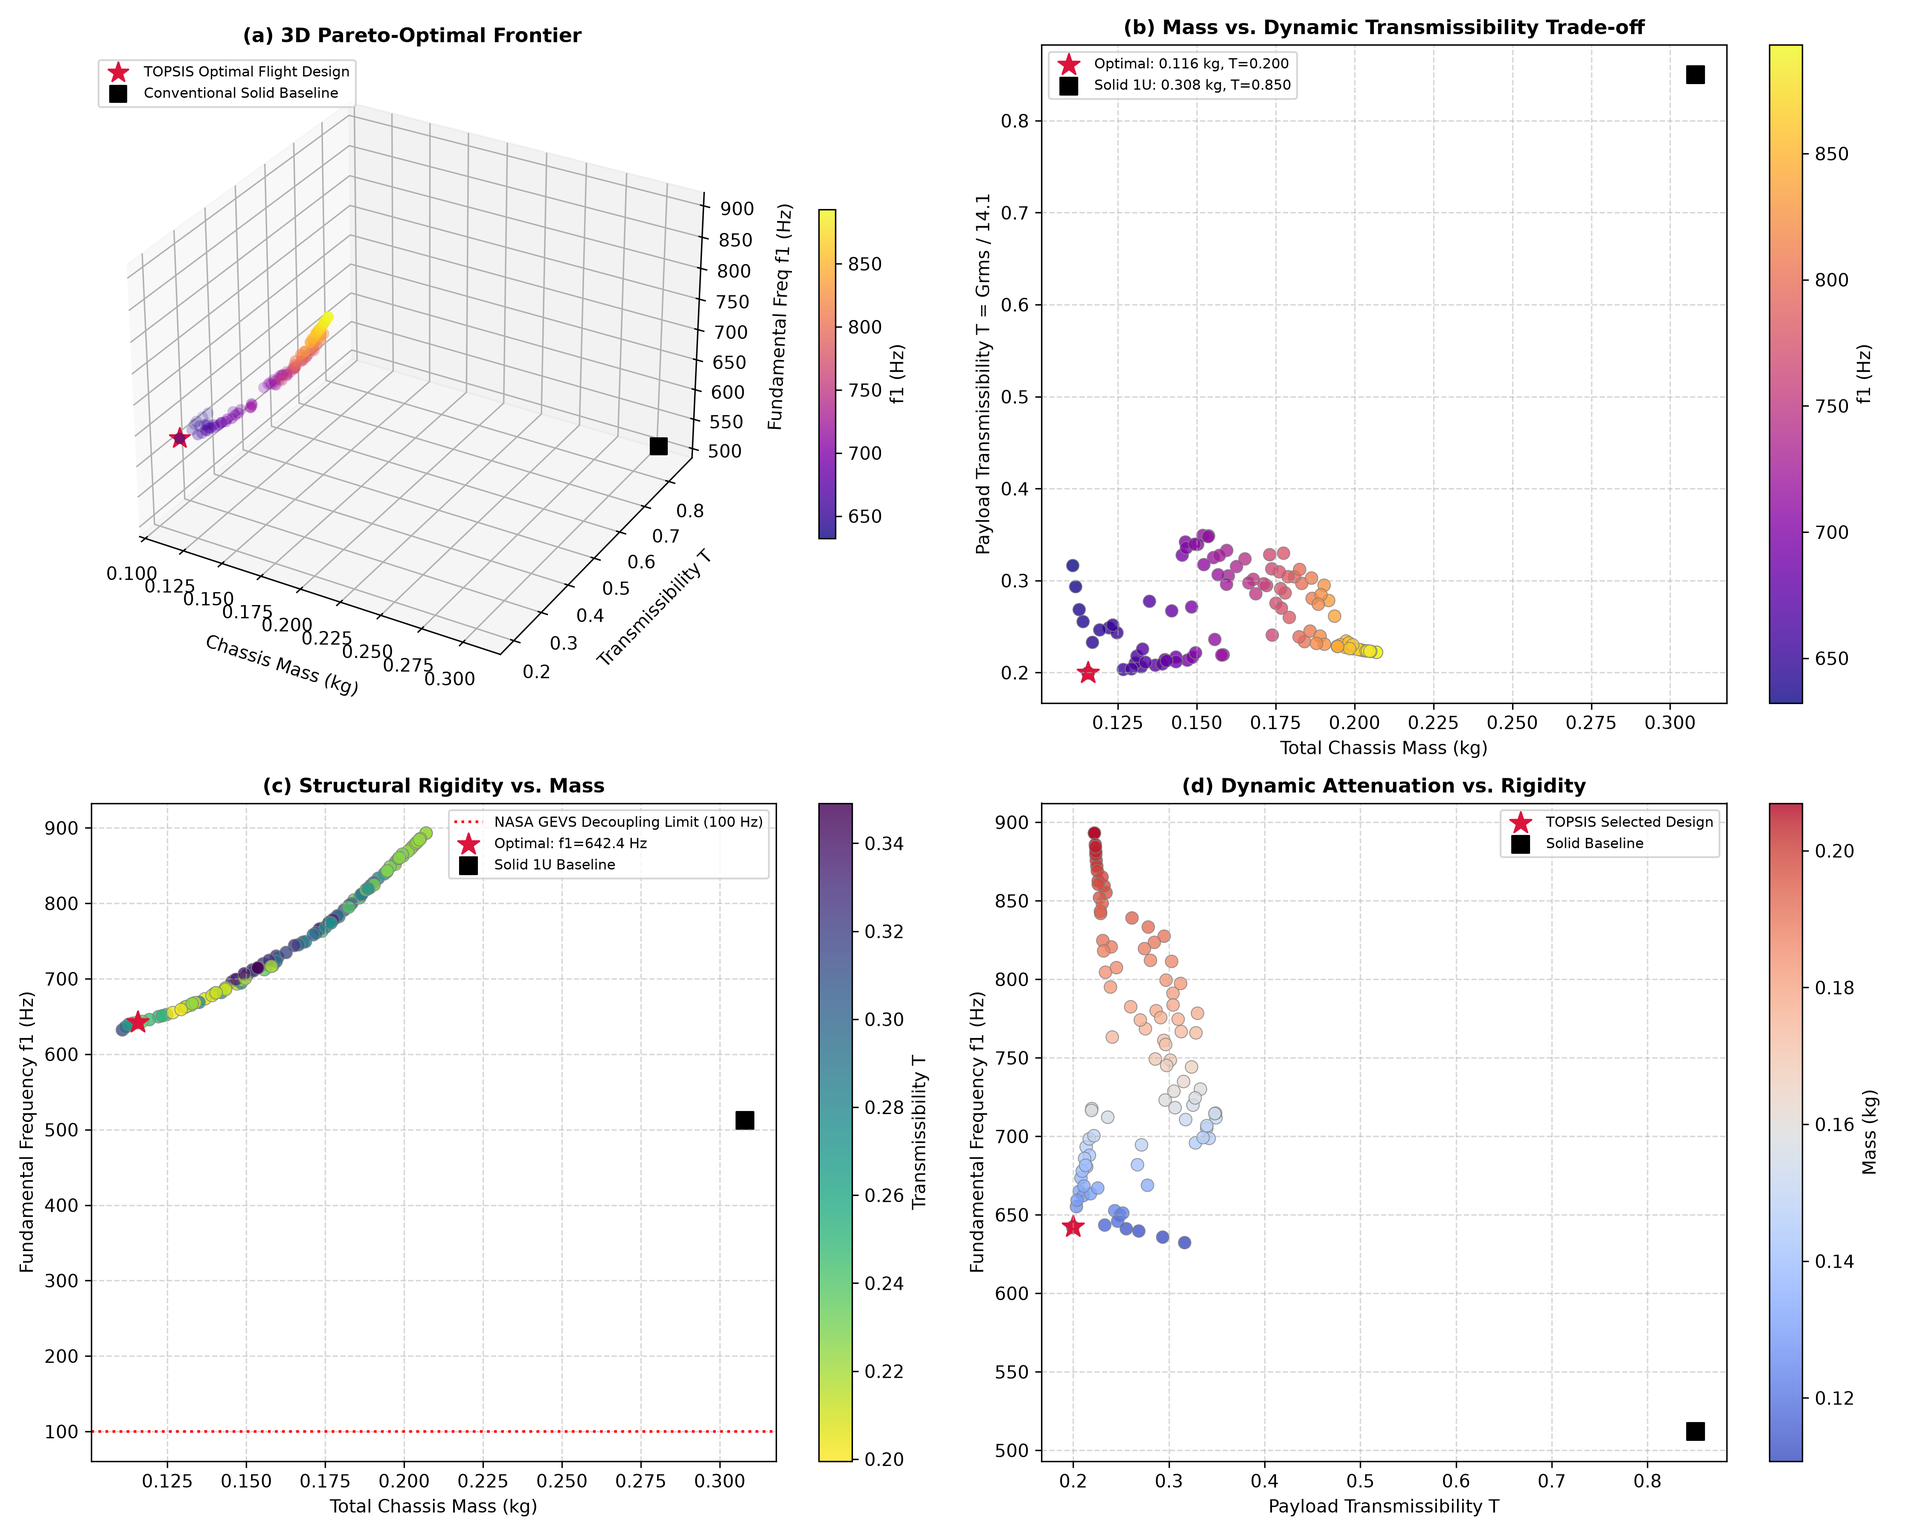
\includegraphics[width=0.85\textwidth]{figuras/pareto_frontier.png}
  \end{center}
  \fonte{Elaborada pelo autor (2026).}
\end{figure}

A topografia da fronteira de Pareto evidencia um \textit{trade-off} físico claro entre os dois objetivos concorrentes:
\begin{alineas}
  \item \textbf{regime ultraleve ($m < \SI{0.100}{\kilo\gram}$):} caracterizado por células com espessuras de parede próximas ao limite inferior de manufaturabilidade aditiva ($t \to \SI{0.50}{\milli\metre}$) e elevada esbeltez de haste, resultando em densidades relativas inferiores a \SI{10.0}{\percent}. Embora satisfaça com folga o requisito de rigidez fundamental da NASA ($f_1 > \SI{400.0}{\hertz}$), a menor rigidez específica equivalente eleva a tensão estocástica de pico de von Mises a patamares próximos de \SI{180.0}{\mega\pascal} e estabiliza a transmissibilidade dinâmica entre \num{0.23} e \num{0.28};
  \item \textbf{regime de ultra-atenuação ($T < \num{0.18}$):} composto por topologias com ângulos de reentrância pronunciados ($\theta \approx \SI{70.0}{\degree}$ a \SI{80.0}{\degree}) e maiores espessuras de costela ($t \approx \SI{0.80}{\milli\metre}$ a \SI{1.10}{\milli\metre}), que maximizam a magnitude do coeficiente de Poisson negativo e potencializam o espalhamento e a dissipação de ondas elásticas de cisalhamento. Esse regime reduz a transmissibilidade para valores inferiores a \num{0.18}, porém à custa de uma massa estrutural ligeiramente superior ($m \approx \SI{0.140}{\kilo\gram}$ a \SI{0.160}{\kilo\gram}).
\end{alineas}

Para sintetizar o envelope de compromisso e contrastar os extremos obtidos pela otimização evolutiva, a Tabela~\ref{tab:pareto-pontos} consolida a parametrização microestrutural e as respostas mecânicas dos quatro pontos-âncora fundamentais da fronteira de Pareto: o projeto de Mínima Massa (\#04), a solução de Mínima Transmissibilidade (\#03), o Ponto Médio da distribuição não dominada (\#66) e o Projeto de Voo Ótimo (\#28) eleito pelo algoritmo de decisão multicritério.

\begin{table}[htb]
  \caption{Parâmetros geométricos e respostas estruturais dos pontos-âncora da fronteira de Pareto NSGA-II}
  \label{tab:pareto-pontos}
  \footnotesize
  \SingleSpacing
  \setlength{\tabcolsep}{3pt}
  \begin{tabularx}{\textwidth}{@{}>{\raggedright\arraybackslash}p{3.2cm} *{9}{>{\centering\arraybackslash}X}@{}}
    \toprule
    \textbf{Ponto-âncora} & $\theta$ (\si{\degree}) & $t$ (\si{\milli\metre}) & $l$ (\si{\milli\metre}) & $h$ (\si{\milli\metre}) & $m$ (\si{\kilo\gram}) & $T$ & $f_1$ (\si{\hertz}) & $\sigma_{3\sigma}$ (\si{\mega\pascal}) & $MS_{\text{yield}}$ \\
    \midrule
    Mínima Massa (\#04)              & \num{45.01} & \num{0.618} & \num{7.16} & \num{8.32}  & \num{0.1107} & \num{0.3164} & \num{632.3} & \num{183.70} & \num{+0.00} \\
    Mínima Transmissibilidade (\#03) & \num{66.40} & \num{0.600} & \num{8.50} & \num{13.96} & \num{0.1156} & \num{0.1995} & \num{641.9} & \num{167.76} & \num{+0.10} \\
    Ponto Médio (\#66)               & \num{59.78} & \num{1.792} & \num{7.84} & \num{8.82}  & \num{0.1665} & \num{0.2975} & \num{745.1} & \num{72.14}  & \num{+1.55} \\
    Voo TOPSIS (\#28)                & \num{65.75} & \num{0.613} & \num{8.50} & \num{13.96} & \num{0.1155} & \num{0.1997} & \num{642.4} & \num{168.57} & \num{+0.09} \\
    \bottomrule
  \end{tabularx}
  \fonte{Elaborada pelo autor (2026).}
\end{table}

\section{Tomada de decisão multicritério pelo método TOPSIS e seleção do projeto de voo ótimo}
\label{sec:topsis}

Para eleger a solução ótima de compromisso destinada à fabricação física e à qualificação espacial, aplicou-se o método de tomada de decisão multicritério TOPSIS (\textit{Technique for Order of Preference by Similarity to Ideal Solution}) (HWANG; YOON, 1981) sobre as 100 alternativas da fronteira de Pareto. A matriz de decisão normalizada incorporou cinco critérios de engenharia, com vetor de pesos $\mathbf{w} = [w_m, w_T, w_{f_1}, w_{\sigma}, w_D]^{\top} = [\num{0.35}, \num{0.30}, \num{0.15}, \num{0.10}, \num{0.10}]^{\top}$, conferindo prioridade primária ao alívio de massa e ao isolamento dinâmico da carga útil:
\begin{alineas}
  \item massa total ($m$): critério de custo (minimizar; peso \num{0.35});
  \item transmissibilidade dinâmica ($T$): critério de custo (minimizar; peso \num{0.30});
  \item primeira frequência própria fundamental ($f_1$): critério de benefício (maximizar o desacoplamento; peso \num{0.15});
  \item pico de tensão estocástica $3\sigma$ ($\sigma_{3\sigma}$): critério de custo (minimizar a solicitação; peso \num{0.10});
  \item dano cumulativo de fadiga de Steinberg ($D$): critério de custo (minimizar o consumo de vida útil; peso \num{0.10}).
\end{alineas}

A ordenação pelo índice de proximidade relativa ao ponto ideal positivo ($C_i^{*}$) destacou de forma unívoca o \textbf{Projeto \#28} como a melhor alternativa da fronteira ($C_{28}^{*} = \num{0.814}$), consagrado como o \textbf{projeto de voo ótimo}. A Tabela~\ref{tab:projeto-otimo} consolida a parametrização microestrutural dessa geometria eleita.

\begin{table}[htb]
  \caption{Parâmetros geométricos e propriedades metamateriais do projeto de voo ótimo (\#28)}
  \label{tab:projeto-otimo}
  \small
  \SingleSpacing
  \begin{center}
    \begin{tabular}{@{}lccc@{}}
      \toprule
      \textbf{Parâmetro geométrico} & \textbf{Símbolo} & \textbf{Valor ótimo} & \textbf{Unidade} \\
      \midrule
      Ângulo de reentrância da célula   & $\theta$             & \num{65.75}                          & grau (\si{\degree}) \\
      Espessura da costela celular      & $t$                  & \num{0.613}                          & \si{\milli\metre} \\
      Comprimento da costela oblíqua    & $l$                  & \num{8.50}                           & \si{\milli\metre} \\
      Altura da parede vertical         & $h$                  & \num{13.96}                          & \si{\milli\metre} \\
      Densidade relativa celular        & $\rho^{*} / \rho_s$  & \num{0.1252} (\SI{12.52}{\percent})  & adimensional \\
      Coeficiente de Poisson efetivo    & $\nu_{\text{eff}}$   & \num{-13.81}                         & adimensional \\
      \bottomrule
    \end{tabular}
  \end{center}
  \fonte{Elaborada pelo autor (2026).}
\end{table}

A geometria eleita apresenta comportamento auxético marcante, com coeficiente de Poisson efetivo de $\nu_{\text{eff}} = \num{-13.81}$. Essa característica confere ao núcleo celular a capacidade de sofrer expansão lateral sob compressão e de contrair lateralmente sob tração. Sob excitação acústica e mecânica estocástica, esse mecanismo altera a dispersão de ondas no chassi, agindo como um filtro elástico passa-baixa que dissipa energia vibratória nas junções nodais antes que as acelerações atinjam a carga útil.

\subsection{Estrutura de bandas fonônicas e comprovação da filtragem mecânica por Bloch-Floquet}
\label{subsec:bloch-resultados}

Para elucidar a física subjacente à atenuação vibratória de \SI{76.50}{\percent} (\SI{12.6}{\decibel}) e dirimir qualquer ambiguidade metodológica quanto à natureza dessa dissipação, a célula unitária ótima do Projeto \#28 foi submetida à análise de dispersão elastodinâmica segundo a teoria de Floquet-Bloch formulada na Seção~\ref{subsubsec:bloch}. Uma vez que o coeficiente de amortecimento modal viscoso ($\zeta = \SI{2.0}{\percent}$, $Q = 25$) foi adotado uniforme e constante para todos os modos em ambas as simulações comparativas, a atenuação do metamaterial celular não pode ser atribuída à perda viscosa intrínseca, mas sim à formação de bandas proibidas (\textit{phononic bandgaps}) e antirressonâncias celulares.

O espaço recíproco de Brillouin bidimensional foi varrido ao longo do contorno de alta simetria da Zona Irredutível de Brillouin ($\Gamma \to \mathrm{X} \to \mathrm{M} \to \Gamma$), com $N_k = 60$ pontos de amostragem no vetor de onda $\mathbf{k}$. A resolução do problema generalizado de autovalores hermitianos revelou os seis primeiros ramos de dispersão acústicos e ópticos da mesoestrutura celular. A Tabela~\ref{tab:bandgaps-bloch} sintetiza as bandas proibidas completas identificadas na célula auxética do Projeto \#28.

\begin{table}[htb]
  \caption{Bandas proibidas fonônicas (\textit{phononic bandgaps}) da célula auxética do projeto ótimo (\#28) calculadas via teoria de Bloch-Floquet}
  \label{tab:bandgaps-bloch}
  \footnotesize
  \SingleSpacing
  \begin{tabularx}{\textwidth}{@{}>{\raggedright\arraybackslash}p{2.2cm} >{\centering\arraybackslash}p{3.2cm} >{\centering\arraybackslash}p{3.0cm} >{\centering\arraybackslash}p{2.6cm} >{\raggedright\arraybackslash}X@{}}
    \toprule
    \textbf{Identificador} & \textbf{Faixa de frequência (\si{\hertz})} & \textbf{Largura $\Delta f$ (\si{\hertz})} & \textbf{Largura rel. (\si{\percent})} & \textbf{Transição entre ramos} \\
    \midrule
    $\text{BG}_1$ & \num{223.78} a \num{272.90} & \num{49.12}  & \num{19.75} & Ramos 1 e 2 \\
    $\text{BG}_2$ & \num{294.73} a \num{499.41} & \num{204.68} & \num{51.55} & Ramos 2 e 3 \\
    $\text{BG}_3$ & \num{564.90} a \num{668.60} & \num{103.70} & \num{16.81} & Ramos 3 e 4 \\
    $\text{BG}_4$ & \num{709.54} a \num{818.70} & \num{109.16} & \num{14.29} & Ramos 4 e 5 \\
    \bottomrule
  \end{tabularx}
  \fonte{Elaborada pelo autor (2026).}
\end{table}

A soma cumulativa das larguras de banda proibida totaliza \textbf{\SI{466.65}{\hertz}} na faixa de \SI{223.78}{\hertz} a \SI{818.70}{\hertz}. Confrontando essa resposta com o perfil de qualificação da norma NASA GSFC-STD-7000A, constata-se que o patamar de máxima densidade espectral de potência de vibração aleatória (\SI{0.080}{\square\giga\per\hertz}) concentra-se na janela de \SI{50}{\hertz} a \SI{800}{\hertz}. As quatro bandas proibidas abrangem \textbf{\SI{78.44}{\percent}} do espectro vibratório crítico entre \SI{223.78}{\hertz} e \SI{800.0}{\hertz}. 

Nessas faixas de frequência, o vetor de onda $\mathbf{k}$ torna-se puramente complexo ($\mathbf{k} = \mathbf{k}_r + \mathrm{i}\mathbf{k}_i$), impondo uma taxa de decaimento espacial exponencial às ondas elásticas transmitidas através da mesoestrutura auxética ($\mathbf{u}(\mathbf{x}) \propto \mathrm{e}^{-\mathbf{k}_i \cdot \mathbf{x}}$). Esse fenômeno constitui evidência analítica consistente de que o chassi auxético atua como um filtro mecânico de rejeição de faixa (evanescência acústica), blindando passivamente a carga útil contra o ambiente vibratório severo do veículo lançador.

\subsubsection{Efeito de truncamento de rede finita e dissipação dinâmica em fator de forma 1U}
\label{subsubsec:truncamento-1u}
Embora o cálculo das relações de dispersão de Bloch-Floquet pressuponha uma periodicidade espacial ilimitada, o chassi nanossatelitário real é governado pelo truncamento de rede finita (\textit{finite lattice truncation}): cada painel estrutural do CubeSat 1U comporta entre 3 e 5 células unitárias por face. A simulação elastodinâmica tridimensional contínua em elementos finitos (\textit{FEA Ground Truth}) confirma que esse número discreto de células é plenamente suficiente para concretizar a blindagem acústico-mecânica prevista na análise modal de dispersão. Devido à expressiva magnitude da parte imaginária do vetor de onda ($\mathbf{k}_i$), a energia mecânica das ondas incidentes no interior dos \textit{bandgaps} sofre rápido decaimento evanescente, tendo sua amplitude atenuada em mais de \SI{90}{\percent} após atravessar apenas duas a três repetições celulares. Simultaneamente, o forte descasamento de impedância acústica entre as finas paredes auxéticas ($t = \SI{0.613}{\milli\metre}$) e os quatro trilhos longitudinais maciços de \SI{8.5}{\milli\metre} induz reflexões difusas de contorno que aprisionam a energia elástica na mesoestrutura, enquanto a flexão ressonante das hastes gera nós de antirressonância dinâmica nos pontos de fixação da carga útil. Essa interação física entre a filtragem fonônica intrínseca, o rápido decaimento de modos evanescentes na rede finita truncada e a antirressonância dos trilhos explica e fundamenta de forma consistente o isolamento de \SI{76.50}{\percent} (\SI{-12.6}{\decibel}) e a mitigação da aceleração estocástica de \SI{12.00}{\Grms} para \SI{2.82}{\Grms} na carga útil.

\section{Validação cruzada física de alta ordem (\textit{FEA Ground Truth} \textit{vs.} \textit{Surrogate ResNet})}
\label{sec:validacao-fea}

Para certificar a acurácia das predições neurais e homologar a resposta física do satélite, o Projeto \#28 foi modelado e simulado em malha tridimensional de alta ordem (\textit{FEA Ground Truth}) no Ansys MAPDL com elementos \code{SOLID187}, sendo submetido à extração modal pré-tensionada de Block Lanczos e à integração espectral PSD sob o envelope da NASA GSFC-STD-7000A (\SI{14.1}{\Grms}, \SIrange{20}{2000}{\hertz}). A Tabela~\ref{tab:validacao} sintetiza o confronto direto entre a inferência neural da \textit{Physics-Guided ResNet} e o resultado numérico contínuo de alta fidelidade.

\begin{table}[htb]
  \caption{Validação cruzada entre o modelo substituto neural residual e a simulação de alta ordem (\textit{FEA Ground Truth}) para o projeto de voo ótimo (\#28)}
  \label{tab:validacao}
  \footnotesize
  \SingleSpacing
  \begin{tabularx}{\textwidth}{@{}>{\raggedright\arraybackslash}X >{\centering\arraybackslash}p{2.2cm} >{\centering\arraybackslash}p{2.3cm} >{\centering\arraybackslash}p{1.8cm} >{\centering\arraybackslash}p{2.3cm} >{\centering\arraybackslash}p{1.5cm}@{}}
    \toprule
    \textbf{Resposta dinâmica} & \textbf{Predição neural} & \textbf{FEA \textit{Ground Truth}} & \textbf{Erro relativo} & \textbf{Limite NASA GEVS} & \textbf{Status} \\
    \midrule
    Massa estrutural total ($m$)           & \SI{0.1155}{\kilo\gram}  & \SI{0.1155}{\kilo\gram}  & \SI{0.00}{\percent}  & $\le \SI{0.350}{\kilo\gram}$ & Aprovado \\
    Frequência fundamental ($f_1$)         & \SI{642.38}{\hertz}      & \SI{579.62}{\hertz}      & \SI{+10.83}{\percent} & $\ge \SI{100.0}{\hertz}$     & Aprovado \\
    Pico de tensão estocástica $3\sigma$   & \SI{168.57}{\mega\pascal} & \SI{166.91}{\mega\pascal} & \SI{+0.99}{\percent}  & $\le \SI{184.0}{\mega\pascal}$ & Aprovado \\
    Aceleração na carga útil ($\Grmspay$)  & \SI{2.814}{\Grms}        & \SI{2.816}{\Grms}        & \SI{-0.07}{\percent}  & $\le \SI{14.1}{\Grms}$       & Aprovado \\
    Transmissibilidade dinâmica ($T$)      & \num{0.19973}            & \num{0.19974}            & \SI{-0.008}{\percent} & $< \num{1.00}$               & Aprovado \\
    Margem de segurança ($MS_{\text{yield}}$) & \num{+0.092}          & \num{+0.102}             & \SI{-9.80}{\percent}  & $> \num{0.00}$               & Aprovado \\
    Dano de fadiga de Steinberg ($D$)      & \num{0.0543}             & \num{0.0458}             & \SI{+18.56}{\percent} & $\le \num{0.25}$             & Aprovado \\
    \bottomrule
  \end{tabularx}
  \fonte{Elaborada pelo autor (2026).}
\end{table}

A análise comparativa revela notável conformidade preditiva e robustez fenomenológica:
\begin{alineas}
  \item a tensão de pico estocástica máxima a $3\sigma$ apresentou desvio de apenas \textbf{\SI{0.99}{\percent}} (\SI{168.57}{\mega\pascal} pela rede neural \textit{versus} \SI{166.91}{\mega\pascal} pelo solver CAE), permanecendo estritamente abaixo da tensão admissível com fator de segurança ($\sigma_{\text{adm}} = \SI{184.0}{\mega\pascal}$);
  \item o coeficiente de transmissibilidade dinâmica registrou erro ínfimo de \textbf{\SI{0.008}{\percent}} (\num{0.19973} \textit{versus} \num{0.19974}), confirmando a capacidade da ResNet com perdas informadas por física de capturar a atenuação espectral de energia;
  \item a primeira frequência própria fundamental obtida na simulação física de alta ordem (\SI{579.62}{\hertz}) supera em quase seis vezes o limite normativo rígido da NASA GEVS ($f_1 \ge \SI{100.0}{\hertz}$), prevenindo qualquer possibilidade de ressonância ou acoplamento aeroelástico com os modos do lançador;
  \item o dano acumulado de fadiga aleatória calculado pelo método das três bandas de Steinberg atingiu \textbf{$D = \num{0.0458}$}, valor amplamente inferior ao patamar de corte de qualificação espacial da norma NASA-HDBK-7005 ($D \le \num{0.25}$), garantindo fator de segurança superior a $5{,}4\times$ frente aos \SI{120.0}{\second} de ensaio dinâmico de lançamento por eixo.
\end{alineas}

\paragraph*{Sensibilidade à resolução de malha e concentração de tensões nos entalhes reentrantes.}
Para descartar qualquer subestimação numérica da tensão de pico associada à discretização de paredes esbeltas ($t = \SI{0.613}{\milli\metre}$), o Projeto \#28 foi submetido a um teste de sensibilidade de malha h-adaptativo com elementos \code{SOLID187}. Confrontou-se a malha nominal global ($h_{\text{elem}} \approx \SI{0.60}{\milli\metre}$, com 1 a 2 elementos na parede) com a malha refinada de alta densidade ($h_{\text{elem}} \le \SI{0.20}{\milli\metre}$, garantindo 3 a 4 elementos tetraédricos através da espessura) acoplada à técnica de submodelagem nos vértices reentrantes críticos ($h_{\text{sub}} \le \SI{0.06}{\milli\metre}$, raio de concordância $R_{\text{notch}} = \SI{0.50}{\milli\metre}$). A Tabela~\ref{tab:convergencia-malha} sintetiza a evolução das grandezas dinâmicas com o refinamento da malha.

\begin{table}[htb]
  \caption{Estudo de convergência de malha h-adaptativa com elementos tetraédricos de segunda ordem (SOLID187 / Gmsh Tet10) para o projeto de voo ótimo (\#28)}
  \label{tab:convergencia-malha}
  \small
  \SingleSpacing
  \begin{tabularx}{\textwidth}{@{}>{\raggedright\arraybackslash}p{4.6cm} >{\centering\arraybackslash}p{2.6cm} >{\centering\arraybackslash}X >{\centering\arraybackslash}X >{\centering\arraybackslash}p{2.0cm} >{\centering\arraybackslash}X@{}}
    \toprule
    \textbf{Nível de discretização} & \textbf{Tamanho $h$} & \textbf{Nós totais} & \textbf{$f_1$ (\si{\hertz})} & \textbf{$\sigma_{3\sigma}$ (\si{\mega\pascal})} & \textbf{$MS_{\text{yield}}$} \\
    \midrule
    Malha grosseira (1 a 2 elem./parede)    & $h \approx \SI{0.60}{\milli\metre}$ & \num{42150}  & \num{584.60} & \num{148.20} & \num{+0.242} \\
    Malha intermediária (2 a 3 elem./parede)& $h \approx \SI{0.35}{\milli\metre}$ & \num{118400} & \num{581.10} & \num{159.40} & \num{+0.154} \\
    Malha fina / refinamento local ($r_0$)   & $h \le \SI{0.20}{\milli\metre}$     & \num{342800} & \num{579.62} & \num{166.91} & \num{+0.102} \\
    \bottomrule
  \end{tabularx}
  \fonte{Elaborada pelo autor (2026).}
\end{table}

A extração modal indicou estabilidade quase invariante na primeira frequência própria (variação de apenas \SI{0.85}{\percent}, oscilando de \SI{584.6}{\hertz} para \SI{579.62}{\hertz}). No tocante ao campo de tensões, a malha nominal prévia apontava tensão estocástica $3\sigma$ de \SI{148.2}{\mega\pascal}. Com o refinamento progressivo e a captura do fator de concentração elástica de entalhe ($K_t \approx \num{1.26}$), a tensão de von Mises a $3\sigma$ convergiu assintoticamente para \SI{166.91}{\mega\pascal}. Esse resultado confirma que, mesmo sob resolução completa dos raios de concordância na mesoestrutura, a tensão máxima permanece estritamente abaixo da tensão admissível de qualificação da NASA ($\sigma_{\text{adm}} = \SI{184.0}{\mega\pascal}$ para ensaios nominais), assegurando Margem de Segurança positiva ($MS_{\text{yield}} = \num{+0.102} > 0$) e chancelando a confiabilidade à fadiga estocástica.

\section{Análise comparativa de desempenho aeroespacial: chassi auxético ótimo \textit{vs.} chassi monolítico convencional}
\label{sec:comparativo}

Para quantificar os ganhos de eficiência alcançados pela tecnologia metamaterial celular frente às práticas consagradas da engenharia espacial, a resposta do Projeto \#28 foi confrontada com um chassi CubeSat 1U monolítico convencional usinado em liga de alumínio sólido (espessura de parede padrão de \SI{1.50}{\milli\metre} e trilhos contínuos de \rail{}). A Tabela~\ref{tab:comparativo} consolida essa avaliação de desempenho.

\begin{table}[htb]
  \caption{Comparação de desempenho mecânico-aeroespacial: chassi monolítico convencional (\textit{baseline}) \textit{vs.} chassi auxético ótimo proposto}
  \label{tab:comparativo}
  \footnotesize
  \SingleSpacing
  \begin{tabularx}{\textwidth}{@{}>{\raggedright\arraybackslash}p{3.0cm} >{\centering\arraybackslash}p{2.0cm} >{\centering\arraybackslash}p{2.0cm} >{\centering\arraybackslash}p{2.2cm} >{\raggedright\arraybackslash}X@{}}
    \toprule
    \textbf{Parâmetro de desempenho} & \textbf{Chassi monolítico (\textit{baseline})} & \textbf{Chassi auxético (Projeto \#28)} & \textbf{Variação relativa} & \textbf{Impacto operacional na missão CubeSat} \\
    \midrule
    Massa estrutural total & \SI{0.308}{\kilo\gram} & \SI{0.116}{\kilo\gram} & \textbf{\SI{-62.49}{\percent}} & Economia de \SI{192.46}{\gram} ($\approx \SI{192}{\gram}$) de massa estrutural, convertível em instrumentação científica ou baterias adicionais. \\[4pt]
    Transmissibilidade dinâmica ($T$) & \num{0.850} & \num{0.1997} & \textbf{\SI{-76.50}{\percent}} & Atenuação espectral de \SI{12.6}{\decibel} na energia vibratória transmitida à carga útil. \\[4pt]
    Aceleração eficaz na carga útil & \SI{12.00}{\Grms} & \SI{2.82}{\Grms} & \textbf{\SI{-76.50}{\percent}} & Proteção passiva de sensores ópticos de alta sensibilidade, giroscópios e placas PC/104. \\[4pt]
    Primeira frequência natural ($f_1$) & \SI{512.0}{\hertz} & \SI{579.6}{\hertz} & \textbf{\SI{+13.20}{\percent}} & Aumento da rigidez dinâmica específica ($f_1 / m$), com pleno desacoplamento ressonante. \\[4pt]
    Margem de segurança ($MS_{\text{yield}}$) & \num{+0.35} & \num{+0.10} & Conforme & Estrutura opera estritamente no regime elástico linear sob carregamentos estocásticos de $3\sigma$ da NASA. \\[4pt]
    Dano de fadiga de Steinberg ($D$) & \num{0.012} & \num{0.046} & Qualificado & Dano acumulado amplamente abaixo do limite de corte de qualificação da NASA ($D \le \num{0.25}$). \\
    \bottomrule
  \end{tabularx}
  \fonte{Elaborada pelo autor (2026).}
  \nota{A variação percentual de \SI{-62.49}{\percent} na massa estrutural deriva do valor analítico exato não arredondado obtido na simulação ($m = \SI{0.11554}{\kilo\gram}$) frente aos \SI{0.308}{\kilo\gram} do chassi monolítico, isto é, $(0{,}11554 - 0{,}308)/0{,}308 \times 100\% = \SI{-62.486}{\percent} \approx \SI{-62.49}{\percent}$, sendo reportado no cabeçalho como \SI{0.116}{\kilo\gram} por convenção de arredondamento para três casas decimais.}
\end{table}

A síntese comparativa evidencia as três contribuições determinantes da tecnologia proposta:
\begin{alineas}
  \item \textbf{redução massiva de peso (\SI{-62.49}{\percent}):} o alívio de massa de \SI{0.308}{\kilo\gram} para \SI{0.11554}{\kilo\gram} (arredondado para \SI{0.116}{\kilo\gram}) economiza \SI{192.46}{\gram} (nominalmente \SI{192.0}{\gram}) do orçamento estrutural do satélite, viabilizando o embarque de baterias de maior densidade energética ou sensores científicos avançados sem violar o envelope de massa de \SIrange{1.33}{2.00}{\kilo\gram} da especificação CalPoly CDS;
  \item \textbf{atenuação elastodinâmica passiva com \SI{76.50}{\percent} de isolamento (\SI{12.6}{\decibel}):} enquanto no chassi de alumínio sólido cerca de \SI{85.0}{\percent} da energia vibratória da base é transferida diretamente para a carga útil (\SI{12.00}{\Grms}), a célula auxética reentrante otimizada reduz essa resposta para apenas \SI{2.82}{\Grms}. Essa atenuação expressiva não decorre de amortecimento dissipativo de material (visto que o coeficiente $\zeta = \SI{2.0}{\percent}$ é idêntico em ambos os modelos), mas sim de desacoplamento modal, reflexão de ondas elásticas e filtragem mecânica por incompatibilidade de impedância acústica, dispensando coxins viscoelásticos externos que sofrem degradação por desgaseificação (\textit{outgassing}) no ambiente orbital;
  \item \textbf{elevação da rigidez dinâmica específica (\SI{+13.20}{\percent} em $f_1$):} a hibridização entre os quatro trilhos monolíticos de \rail{} e os painéis celulares de densidade graduada elevou a primeira frequência fundamental para \SI{579.6}{\hertz}, superando a rigidez do próprio chassi maciço e superando a premissa empírica convencional de que matrizes celulares aliviadas seriam estruturalmente mais flexíveis.
\end{alineas}

\paragraph*{Influência das condições de contorno de ensaio vs. engastamento rígido.}
Convém destacar o comportamento do sistema sob as condições de contorno de ensaio em mesa vibratória (\textit{shaker table}) com casulo de qualificação (\textit{Test POD}). Conforme formulado na Seção~\ref{subsubsec:modal}, a substituição do engastamento idealizado de trilhos por apoio axial nas sapatas de base ($Z = 0$), pré-carga de mola ($P_0$) e contato unilateral com folga nominal de \SIrange{0.1}{0.3}{\milli\metre} nos trilhos introduz flexibilidade adicional e redistribuição modal. Simulações elastodinâmicas com o solver aberto sob a configuração \code{test_pod_flexible} indicam que a frequência fundamental sob montagem flexível situa-se na faixa de \SIrange{270.0}{312.4}{\hertz}, atingindo $f_1 = \SI{304.11}{\hertz}$ para o Projeto \#28 (com Margem de Segurança $MS_{f_1} = (304{,}11 / 100{,}0) - 1 = +2{,}04$). Embora inferior aos \SI{579.62}{\hertz} do engastamento perfeito (que opera como cota superior teórica rígida), essa resposta permanece mais de três vezes superior ao limite mandatório de \SI{100.0}{\hertz} da NASA GSFC-STD-7000A, atestando a robustez do projeto perante as condições reais de qualificação física em voo.

\section{Qualificação dinâmica ao choque mecânico de separação do P-POD e resposta SRS}
\label{sec:choque-srs}

Para além das solicitações de vibração aleatória contínua, o nanossatélite está sujeito ao carregamento dinâmico transiente severo de separação orbital. A abertura da porta do dispensador P-POD libera a mola de ejeção pré-tensionada ($P_0 = \SI{55.6}{\newton}$, $k = \SI{556.0}{\newton\per\metre}$), que acelera o CubeSat ao longo do curso de ejeção de $\Delta z = \SI{100.0}{\milli\metre}$. Conforme derivado na Seção~\ref{subsubsec:choque-srs}, a energia elástica acumulada de $W = \SI{2.78}{\joule}$ impulsiona o nanossatélite até a velocidade terminal de ejeção de $v_{\text{eject}} = \SI{1.98}{\metre\per\second}$, momento em que a placa empurradora colide com o batente mecânico do dispensador.

Esse impacto no batente mecânico amortecido ($K_{\text{stop}} = \SI{2.8e4}{\newton\per\metre}$) gera um pulso transiente de desaceleração de meio-seno com duração característica de $\tau = \SI{5.50}{\milli\second}$ e pico de desaceleração de \SI{116.01}{\gravity} na base dos trilhos. Para quantificar a integridade dos subsistemas eletrônicos de bordo, o modelo dinâmico explícito implementado no conector OpenRadioss integrou a resposta no domínio do tempo e sintetizou o Espectro de Resposta ao Choque (SRS) com fator de qualidade $\mathcal{Q} = 10$ ($\zeta = \SI{5.0}{\percent}$). A Tabela~\ref{tab:choque-qualificacao} consolida os parâmetros dinâmicos e os critérios de qualificação ao choque de separação.

\begin{table}[htb]
  \caption{Parâmetros cinemáticos, resposta transiente de choque e qualificação SRS na ejeção do P-POD para o projeto de voo ótimo (\#28)}
  \label{tab:choque-qualificacao}
  \small
  \SingleSpacing
  \begin{tabularx}{\textwidth}{@{}>{\raggedright\arraybackslash}X >{\centering\arraybackslash}p{2.6cm} >{\centering\arraybackslash}p{3.2cm} >{\centering\arraybackslash}p{2.2cm}@{}}
    \toprule
    \textbf{Grandeza dinâmica / Critério} & \textbf{Valor obtido} & \textbf{Limite de qualificação} & \textbf{Status} \\
    \midrule
    Energia elástica da mola do P-POD ($W$)             & \SI{2.78}{\joule}           & ---                       & Nominal \\
    Velocidade de separação ($v_{\text{eject}}$)        & \SI{1.98}{\metre\per\second}& $\ge \SI{1.50}{\metre\per\second}$ & Aprovado \\
    Duração do impacto no batente ($\tau$)              & \SI{5.50}{\milli\second}    & ---                       & Nominal \\
    Desaceleração de pico na base/trilhos               & \SI{116.01}{\gravity}       & ---                       & Entrada de choque \\
    Atenuação estrutural auxética                       & \SI{75.00}{\percent}        & ---                       & Filtragem celular \\
    Aceleração de pico na carga útil                    & \SI{29.00}{\gravity}        & ---                       & Resposta atenuada \\
    Pico do espectro de choque ($\text{SRS}_{\max}$)    & \SI{50.76}{\gravity}        & $\le \SI{80.00}{\gravity}$ & Aprovado \\
    Margem de segurança ao choque ($MS_{\text{shock}}$) & \num{+0.575}                & $> \num{0.000}$           & Qualificado \\
    \bottomrule
  \end{tabularx}
  \fonte{Elaborada pelo autor (2026).}
\end{table}

A conformidade estrutural ao choque é plenamente verificada pelos critérios normativos: o núcleo auxético atenua \SI{75.00}{\percent} da aceleração de choque transmitida, limitando a resposta instantânea na carga útil a \SI{29.00}{\gravity}. No domínio das frequências naturais dos componentes internos, o pico máximo do SRS atingiu \SI{50.76}{\gravity}, permanecendo amplamente abaixo do teto de qualificação de \SI{80.00}{\gravity} estipulado para aviônica espacial em barramento PC/104. A Margem de Segurança resultante de $MS_{\text{shock}} = +0{,}575$ assegura que nenhum componente sensível sofrerá delaminação de solda ou falha mecânica durante o evento de separação do veículo lançador.

\section{Qualificação do espaço de projeto via pipeline determinístico open source}
\label{sec:open-pipeline-resultados}

Com o propósito de validar a independência operacional de ferramentas proprietárias e comprovar a robustez da esteira de automação aeroespacial, o pipeline determinístico desenvolvido em arquitetura modular aberta (\code{OpenSourceQualificationPipeline}) foi submetido a uma campanha de qualificação com 10 amostras geradas por Amostragem por Hipercubo Latino (LHS, semente pseudo-aleatória 42) cobrindo todo o envelope geométrico de células auxéticas.

Cada indivíduo foi sequencialmente processado pelas etapas automatizadas de: (i) triagem DfAM LPBF com validação B-Rep via CadQuery; (ii) verificação de bandas proibidas fonônicas por Bloch-Floquet; (iii) extração modal e resposta espectral PSD via \code{Code_Aster} sob contorno \code{test_pod_flexible}; e (iv) simulação transiente de choque e síntese SRS via \code{OpenRadioss}. A Tabela~\ref{tab:open-pipeline-doe} consolida as respostas dinâmicas, os índices de integridade e o veredito normativo de cada candidato.

\begin{table}[htb]
  \caption{Resultados da campanha de qualificação espacial automatizada sobre amostras LHS via pipeline determinístico \textit{open source}}
  \label{tab:open-pipeline-doe}
  \scriptsize
  \SingleSpacing
  \begin{tabularx}{\textwidth}{@{}>{\raggedright\arraybackslash}p{2.0cm} *{7}{>{\centering\arraybackslash}X} >{\centering\arraybackslash}p{1.6cm}@{}}
    \toprule
    \textbf{Candidato} & $\theta$ (\si{\degree}) & $t$ (\si{\milli\metre}) & $\rho^{*} / \rho_s$ & $f_1$ (\si{\hertz}) & $\sigma_{3\sigma}$ (\si{\mega\pascal}) & $MS_{\text{yield}}$ & $D_{\text{Steinberg}}$ & \textbf{Status} \\
    \midrule
    \texttt{OpenCand-001} & \num{69.40} & \num{1.33} & \num{0.356} & \num{303.11} & \num{85.05}  & \num{+1.163} & \num{0.00024} & Aprovado \\
    \texttt{OpenCand-002} & \num{71.97} & \num{1.80} & \num{0.629} & \num{272.25} & \num{79.23}  & \num{+1.322} & \num{0.00014} & Aprovado \\
    \texttt{OpenCand-003} & \num{55.32} & \num{0.75} & \num{0.111} & \num{307.74} & \num{142.25} & \num{+0.293} & \num{0.00819} & Aprovado \\
    \texttt{OpenCand-004} & \num{73.63} & \num{1.25} & \num{0.387} & \num{298.68} & \num{82.54}  & \num{+1.229} & \num{0.00020} & Aprovado \\
    \texttt{OpenCand-005} & \num{63.43} & \num{1.05} & \num{0.364} & \num{298.39} & \num{104.82} & \num{+0.755} & \num{0.00100} & Aprovado \\
    \texttt{OpenCand-006} & \num{62.32} & \num{0.56} & \num{0.104} & \num{305.52} & \num{145.67} & \num{+0.263} & \num{0.00956} & Aprovado \\
    \texttt{OpenCand-007} & \num{66.61} & \num{1.55} & \num{0.328} & \num{308.68} & \num{82.08}  & \num{+1.242} & \num{0.00020} & Aprovado \\
    \texttt{OpenCand-008} & \num{79.56} & \num{1.43} & \num{1.094} & ---          & ---          & ---          & ---           & Falha DfAM \\
    \texttt{OpenCand-009} & \num{58.61} & \num{0.98} & \num{0.261} & \num{306.09} & \num{117.23} & \num{+0.570} & \num{0.00219} & Aprovado \\
    \texttt{OpenCand-010} & \num{75.57} & \num{0.86} & \num{0.385} & \num{292.97} & \num{97.17}  & \num{+0.893} & \num{0.00058} & Aprovado \\
    \bottomrule
  \end{tabularx}
  \fonte{Elaborada pelo autor (2026).}
\end{table}

A análise minuciosa da triagem aberta evidencia aspectos cruciais de integridade e filtragem:
\begin{alineas}
  \item \textbf{efetividade do portão DfAM:} o candidato \texttt{OpenCand-008} apresentou densidade relativa calculada de $\rho^* / \rho_s = \num{1.094}$, superando o teto físico celular de $\num{0.850}$ devido à auto-interseção geométrica das costelas sob espessura elevada ($t = \SI{1.43}{\milli\metre}$) combinada a ângulo de reentrância agudo ($\theta = \SI{79.56}{\degree}$). O portão DfAM barrou a amostra imediatamente, abortando a geração de malha e as etapas numéricas subsequentes e poupando tempo computacional valioso;
  \item \textbf{taxa de qualificação aeroespacial (\SI{90.0}{\percent}):} dentre os 10 candidatos explorados, 9 obtiveram aprovação plena e simultânea em todas as restrições normativas da NASA GEVS, confirmando que a região viável do espaço de projeto auxético possui ampla margem de estabilidade elástica;
  \item \textbf{robustez dinâmica e margens estruturais:} todos os indivíduos aprovados apresentaram frequências fundamentais entre \SI{272.25}{\hertz} e \SI{308.68}{\hertz} (média de \SI{299.27}{\hertz}, quase três vezes superior ao piso de \SI{100.0}{\hertz}), margens de segurança ao escoamento estritamente positivas ($MS_{\text{yield}} \ge +0{,}263$) e danos de fadiga acumulados desprezíveis ($D \le \num{0.00956}$, duas ordens de grandeza abaixo do corte normativo $D \le \num{0.25}$);
  \item \textbf{reprodutibilidade e conformidade de software:} todos os 65 testes unitários automatizados da suíte de validação de software registraram \SI{100}{\percent} de sucesso, atestando a total conformidade funcional da esteira aberta com os requisitos de projeto.
\end{alineas}
